\documentclass{standalone}
\usepackage{tikz,color}
\begin{document}
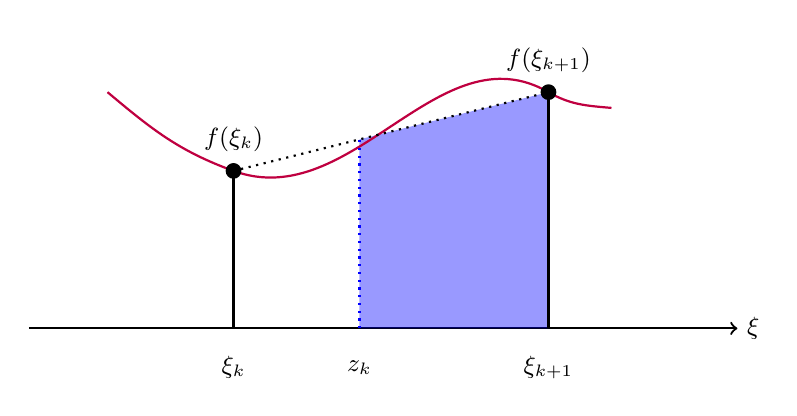
\begin{tikzpicture}[scale=2]

\draw [thick, ->] (-0.5,0) to (4,0);
\node at (4,0) [right] {\small{$\xi$}};

\path [fill=blue ,opacity=0.4]
plot [domain=1.6:2.8, samples=50, thick ] ( {\x}, {1 + (\x-0.8)*0.25)})
|- (1.6,0);

\draw [purple, thick] (0,1.5) to [out=-40,in=160] (0.8,1);
\draw [purple, thick] (0.8,1) to [out=-20,in=150] (2.8,1.5);
\draw [purple, thick] (2.8,1.5) to [out=-30,in=175] (3.2,1.4);

\node at (0.8,-0.25) {\small{$\xi_k$}};
\node at (1.6,-0.25) {\small{$z_k$}};
\node at (2.8,-0.25) {\small{$\xi_{k+1}$}};

\node at (0.8, 1.2) {\small{$f(\xi_k)$}};
\node at (2.8, 1.7) {\small{$f(\xi_{k+1})$}};

\draw [dotted, thick] (0.8,1) -- (2.8,1.5);
\draw [ thick] (0.8,0) -- (0.8,1);
\draw [ thick] (2.8,0) -- (2.8,1.5);
\draw [blue,dotted, thick] (1.6,0) -- (1.6,1.2);

\fill(0.8,1) circle [ radius=0.05];
\fill(2.8,1.5) circle [ radius=0.05];

\end{tikzpicture}
\end{document}
